\pdfbookmark{Общая характеристика работы}{characteristic}             % Закладка pdf
\section*{Общая характеристика работы}

\newcommand{\actuality}{\pdfbookmark[1]{Актуальность}{actuality}\underline{\textbf{\actualityTXT}}}
\newcommand{\progress}{\pdfbookmark[1]{Разработанность темы}{progress}\underline{\textbf{\progressTXT}}}
\newcommand{\aim}{\pdfbookmark[1]{Цели}{aim}\underline{{\textbf\aimTXT}}}
\newcommand{\tasks}{\pdfbookmark[1]{Задачи}{tasks}\underline{\textbf{\tasksTXT}}}
\newcommand{\aimtasks}{\pdfbookmark[1]{Цели и задачи}{aimtasks}\aimtasksTXT}
\newcommand{\novelty}{\pdfbookmark[1]{Научная новизна}{novelty}\underline{\textbf{\noveltyTXT}}}
\newcommand{\influence}{\pdfbookmark[1]{Практическая значимость}{influence}\underline{\textbf{\influenceTXT}}}
\newcommand{\methods}{\pdfbookmark[1]{Методология и методы исследования}{methods}\underline{\textbf{\methodsTXT}}}
\newcommand{\defpositions}{\pdfbookmark[1]{Положения, выносимые на защиту}{defpositions}\underline{\textbf{\defpositionsTXT}}}
\newcommand{\reliability}{\pdfbookmark[1]{Достоверность}{reliability}\underline{\textbf{\reliabilityTXT}}}
\newcommand{\probation}{\pdfbookmark[1]{Апробация}{probation}\underline{\textbf{\probationTXT}}}
\newcommand{\contribution}{\pdfbookmark[1]{Личный вклад}{contribution}\underline{\textbf{\contributionTXT}}}
\newcommand{\publications}{\pdfbookmark[1]{Публикации}{publications}\underline{\textbf{\publicationsTXT}}}



\textbf{Актуальность темы исследования.}

Тематическое моделирование --- это обширное направление исследований в области автоматической обработки текстов. Тематическая модель коллекции текстовых документов определяет, к каким темам относится каждый документ и из каких слов состоит каждая тема. В отличие от обычных методов кластеризации, тематическая модель может относить документ не к одному кластеру-теме, а к нескольким, то есть  она производит <<мягкую кластеризацию>>, причём не только документов, но и слов.

Обычно тематические модели относят к методам машинного обучения <<без учителя>>, поскольку они не требуют размеченных обучающих выборок. Это позволяет использовать тематическое моделирование в тех случаях, когда никаких дополнительных данных, кроме собственно текстовой коллекции, не имеется, например, для информационного поиска в больших текстовых массивах, для анализа специализированных текстов или текстов на редких языках, для анализа больших массивов текстоподобных данных, таких как программный код, тексты песен, банковские транзакции, географические данные, музыкальные произведения.

Результатом вероятностного тематического моделирования является конечное множество \textit{тем}, каждая из которых описывается вероятностным распределением на множестве слов. Важным свойством темы является её интерпретируемость. Слова, имеющие большую вероятность в данной теме, должны относиться к одной предметной области и быть семантически связанными. Тема считается интерпретируемой, если, рассматривая наиболее частотные слова темы, эксперт может сказать, о чём эта тема, и дать ей определённое название~\cite{rtl}. Если все темы (или почти все) интерпретируемые, то о такой модели говорят, что она в целом является интерпретируемой. В таком случае модель может быть полезна для понимания тематической структуры коллекции. Интерпретируемость является трудно формализуемой характеристикой. Существуют различные экспертные и вычислительные методики её количественного оценивания \cite{newman2010automatic}.

Развитие вероятностного тематического моделирования началось с работы Т.Хофманна \cite{hofmann1999}, в которой была предложена модель вероятностного латентного семантического анализа (Probabilistic Latent Semantic Analysis, PLSA). Построение тематической модели является некорректно поставленной задачей стохастического матричного разложения, которая имеет бесконечное множество решений. Для доопределения постановки задачи и выбора наиболее подходящего решения необходимо вводить дополнительные ограничения на модель. Следующей важной вехой стала модель латентного размещения Дирихле (Latent Dirichlet Allocation, LDA) \cite{blei2003latent}, основанная на байесовской регуляризации искомых дискретных распределений с помощью априорных распределений Дирихле. В последующие годы на основе PLSA и LDA были разработаны сотни специализированных моделей, отличающихся способами регуляризации, структурой исходных данных и матричного разложения \cite{daud10knowledge,blei2012,fntir2017applications}.

Аддитивная регуляризация тематических моделей (ARTM) позволяет комбинировать регуляризаторы для создания моделей с заданными свойствами \cite{vorontsov2014additive,voron15mlj}. Это многокритериальный подход, основанный на оптимизации взвешенной суммы основного критерия (логарифма правдоподобия) и некоторого количества дополнительных критериев-регуляризаторов. Многокритериальный подход является ответом на практическую потребность строить модели, обладающие целым рядом необходимых свойств одновременно \cite{kochedykov2017fast}.

Соответственно, в каждой конкретной задаче тематического моделирования может быть много не только оптимизационных критериев, но и метрик качества, с помощью которых валидируется (оценивается) построенная модель. В частности, в \cite{voron15mlj,voron15mlj} было показано, что комбинирование регуляризаторов сглаживания, разреживания, декоррелирования и отбора тем позволяет одновременно улучшить несколько метрик качества (разреженность, различность и интерпретируемость тем) без заметного ухудшения основного критерия правдоподобия (или перплексии) модели. Тематические модели для разведочного информационного поиска, в дополнение к этим свойствам, должны быть также мультимодальными (учитывать не только слова, но и биграммы, теги, категории, авторство документов) и иерархическими (разделять крупные темы на более мелкие подтемы) \cite{ianina2019regularized}. Построение таких моделей требует не только выбора множества модальностей и регуляризаторов, но и подбора различных гиперпараметров.

На основе теории аддитивной регуляризации тематических моделей

была разработана библиотека тематического моделирования с открытым кодом BigARTM \cite{vorontsov2015bigartm,frei2016parallel}.

Свойство аддитивности регуляризаторов позволило реализовать в BigARTM модульный подход, когда пользователь выбирает из библиотеки нужный ему набор регуляризаторов для построения модели с требуемыми свойствами.

Возможность конструирования новых композитных моделей из <<готовых блоков>> существенно отличает BigARTM от других средств тематического моделирования, основанных на теории байесовского обучения, в которой каждая новая модель требует проведения уникальных математических выкладок (байесовского вывода) и, как следствие, разработки нового программного кода.

Несмотря на модульность, гибкость, масштабируемость и высокую производительность \cite{kochedykov2017fast}, практическое применение библиотеки BigARTM наталкивается на ряд трудностей. Пользователь должен хорошо разбираться в теории ARTM, чтобы грамотно выбрать стратегию регуляризации, то есть последовательность включения регуляризаторов, затем подобрать число тем, коэффициенты регуляризации для каждого регуляризатора и другие гиперпараметры. Эта работа связана с проведением серий вычислительных экспериментов, которые требуют тщательного планирования, журнализации, валидации, визуализации и критического осмысления промежуточных результатов. Таким образом, BigARTM перекладывает на пользователя значительный объём работы, требующей пристального внимания и высокой квалификации.

Актуальной задачей является создание технических средств для автоматизации экспериментов по построению аддитивно регуляризованных тематических моделей, их валидации и выбора лучшей модели по заданной совокупности метрик качества.

\textbf{Степень разработанности темы исследования.}

Тематическое моделирование является полезным инструментом в цифровых гуманитарных исследованиях (digital humanities) \cite{grimmer2013text,paakkonen2020humanistic}. Однако процессы построения, валидации и выбора тематических моделей практически не алгоритмизированы \cite{paakkonen2020humanistic}. Большое прикладное значение имеет разработка новых методов визуализации, автоматической валидации и выбора моделей \cite{dh_sea}.

Также исследователи сталкиваются с неустойчивостью \cite{mantyla2018measuring} и неинтерпретируемостью тем \cite{boydcare}. Известно, что настройка гиперпараметров модели может повысить её устойчивость \cite{agrawal2018wrong}, однако на практике она выполняется редко, и для неё нет единой принятой методологии  \cite{agrawal2018wrong,chen2016survey}.

Настройка гиперпараметров может помочь и с интерпретируемостью тем, особенно в рамках подхода ARTM. Известные регуляризаторы, такие как регуляризатор декоррелирования, способствуют повышению различности и интерпретируемости тем \cite{popov_hier}; также можно использовать  регуляризатор, напрямую оптимизирующий заданный критерий, как это было сделано в \cite{4keys} для критерия средней когерентности тем.

К сожалению, интерпретируемости трудно дать формальное определение. Попытки определить плохие темы через расстояние до известных <<мусорных>> тем или через низкие значения когерентности дают лишь срез проблематичных тем и имеют ограниченную область применимости \cite{boydcare}. Системный подход к измерению интерпретируемости предполагает оценивание каждой темы по нескольким критериям качества \cite{fan2019assessing}.

Таким образом, принятые методологии перекладывают ответственность за подбор гиперпараметров на исследователя; при этом процедура подбора остаётся нерегламентированной, что создаёт высокий барьер входа для неспециалистов.

В~обзорной монографии \cite{fntir2017applications} подчёркивается важность снижения порога входа и более жёсткой регламентации процесса моделирования: <<первоочередная исследовательская задача в тематическом моделировании... сделать его более доступным>>.

Мы видим, что важными нерешёнными проблемами являются: обеспечение  интерпретируемости моделей, подбор гиперпараметров и стандартизация процесса построения тематической модели для широкого класса пользовательских прикладных задач.

{\aim} данного диссертационного исследования является разработка и реализация технологии построения интерпретируемых аддитивно регуляризованных тематических моделей, применимых для решения широкого класса задач тематического моделирования.

Для~достижения поставленной цели решаются следующие {\tasks}.

\begin{enumerate}[beginpenalty=10000] % https://tex.stackexchange.com/a/476052/104425

  \item Реализация, эмпирическое исследование и улучшение автоматически вычисляемых критериев интерпретируемости тематических моделей, в том числе нового критерия внутритекстовой когерентности.

  \item Разработка методологии и средств автоматизации проведения экспериментов по подбору стратегии регуляризации и выбору гиперпараметров тематической модели.

  \item Проектирование архитектуры библиотеки TopicNet с открытым кодом на GitHub для реализации данной методологии. Разработка и реализация интерфейсов, обеспечивающих создание пользовательских регуляризаторов и метрик качества в TopicNet.

  \item Поиск универсального <<рецепта>> построения аддитивно регуляризованных тематических моделей, превосходящих LDA по совокупности критериев качества, применение которого не требовало бы от пользователя знания теории ARTM.

  \item Решение прикладных задач с использованием разработанной библиотеки TopicNet, в частности, задачи кластеризации интентов в текстовой коллекции обращений клиентов в контактный центр.

\end{enumerate}

\textbf{Научная новизна.}

Предложена новая методология многокритериального выбора моделей на основе концепций <<дерева экспериментов>>, <<кубов гиперпараметров>> и <<рецептов моделирования>> в рамках теории аддитивной регуляризации тематических моделей (ARTM).

Разработан универсальный <<рецепт>> построения аддитивно регуляризованных тематических моделей, превосходящих LDA по совокупности критериев качества.

Предложен новый способ построения иерархических тематических моделей с разными весами модальностей на разных уровнях иерархии.

\textbf{Теоретическая значимость.}

Работа вносит вклад в развитие теории аддитивной регуляризации тематических моделей (ARTM), предоставляя исследователям удобную инструментальную среду, позволяющую накопить эмпирический материал для изучения стратегий регуляризации и их влияния на качество тематических моделей при многокритериальном оценивании. Вводятся понятия внутритекстовой когерентности, относительных и абсолютных коэффициентов регуляризации, фактора балансировки, дерева экспериментов, куба гиперпараметров, рецепта моделирования.

\textbf{Практическая значимость.}

Предложенные подходы и методы реализованы в библиотеке тематического моделирования с открытым кодом TopicNet, которая может быть использована и уже используется для решения различных прикладных задач анализа текстовых и транзакционных данных. Реализованные в библиотеке концепции дерева экспериментов, куба гиперпараметров и рецепта моделирования позволяют находить, сохранять и распространять в сообществе исследователей удачные приёмы решения прикладных задач тематического моделирования.

Показано, что использование относительных коэффициентов регуляризации обеспечивает возможность переноса стратегии обучения тематической модели на другие текстовые коллекции: один и тот же набор значений относительных коэффициентов регуляризации и/или весов модальностей может быть использован для различных прикладных задач. В случае, когда непосредственный перенос численных значений нецелесообразен из-за специфики новой коллекции, относительные коэффициенты облегчают подбор оптимальных значений, поскольку они находятся в диапазоне $[0, 1]$ и интерпретируются как степень воздействия регуляризатора на модель в сравнении с основным критерием логарифмированного правдоподобия.

Предложенные в данной работе и реализованные в TopicNet механизмы были успешно применены для решения ряда прикладных задач:

для кластеризации интентов в текстовой коллекции обращений клиентов в контактный центр \cite{popov_hier},

для анализа банковских транзакционных данных \cite{egorov2019topic} и других.

{\methods} В работе использованы методы теории вероятностей, численной оптимизации, автоматической обработки текстов, машинного обучения, вероятностного тематического моделирования. Экспериментальное исследование проводится на языке Python; опубликованная на GitHub библиотека TopicNet, подытоживающая результаты исследования, открыта для свободного использования и удовлетворяет принципам воспроизводимости результатов.

{\defpositions}

\begin{enumerate}[beginpenalty=10000] % https://tex.stackexchange.com/a/476052/104425

\item

    Разработана методология построения аддитивно регуляризованных тематических моделей, обеспечивающая формирование <<рецептов моделирования>> с автоматизированным подбором гиперпараметров по множеству критериев и отличающаяся использованием относительных коэффициентов регуляризации и кубов гиперпараметров.

\item

    Выстроена архитектура библиотеки TopicNet, обеспечивающая программную реализацию данной методологии и отличающаяся использованием удобного языка описания кубов гиперпараметров и возможностью создания пользовательских регуляризаторов и метрик качества на языке Python.

\item

    Создан универсальный рецепт моделирования, обеспечивающий многокритериальный выбор тематических моделей для широкого класса задач, отличающийся предварительной настройкой куба гиперпараметров по набору разнородных задач тематического моделирования.

\item

    Выполнена программная реализация нового критерия когерентности, обеспечивающая его эффективное вычисление и отличающаяся более полным использованием данных о сочетаемости слов внутри текстовых документов.

%\item

%    Программная реализация псевдорегуляризатора в библиотеке TopicNet, обеспечивающего быстрое однопроходное вычисление тематических векторных представлений документов и улучшение качества тематической модели по множеству критериев.

\end{enumerate}

{\reliability} полученных результатов обеспечивается вычислительными экспериментами на реальных текстовых коллекциях. Методика и результаты подробно описаны в тексте работы. Разработанный код библиотеки TopicNet и проведённых экспериментов находится в открытом доступе, что обеспечивает воспроизводимость результатов.

{\probation}

Основные результаты диссертации докладывались на следующих конференциях и семинарах:

\begin{itemize}

    \item Международная конференция по компьютерной лингвистике <<Диалог>>, Москва, 1 июня 2018.

    \item International Conference Recent Advances in Natural Language Processing (RANLP), Варна, 3 сентября 2019.

    \item Открытая лекция в рамках образовательного проекта Физтех.Рост, Долгопрудный, 18 октября 2019.

    \item Открытый научный семинар <<Методы анализа текстов>>, Москва, 28 марта 2018.

    \item Открытый научный семинар <<Презентация TopicNet>>, Москва, 10 августа 2019.

    \item OpenTalks.AI~--- ведущая открытая конференция по искусственному интеллекту, Москва, 20 февраля 2020 года.

    \item International Conference on Language Resources and Evaluation (LREC), Марсель (должна была состояться в мае 2020).

\end{itemize}

{\contribution} Личный вклад диссертанта в работы, выполненные с

соавторами, заключается в следующем:

\begin{itemize}

    \item В \cite{intracoh} предложен метод генерации полусинтетической выборки, проведены эксперименты по анализу репрезентативности высокочастотных слов в темах.

    \item В \cite{popov_hier} выполнена реализация иерархической тематической модели средствами библиотеки TopicNet; предложен метод разделения слов и $n$-грам по функциональному назначению; предложены методы анализа ошибок моделирования; выполнены эксперименты с относительными коэффициентами регуляризации.

    \item В \cite{bulatov2020topicnet} описана архитектура библиотеки TopicNet, концепция кубов гиперпараметров и дерева эксперимента, методы отбора моделей и связанный с ними специализированный язык описания кубов; проведена часть экспериментов, связанная с GenSim и с различностью тем.

    \item В \cite{thetaless} предложена адаптация псевдорегуляризатора для библиотеки TopicNet и выполнена его программная реализация; проведена связанная с этим часть экспериментов.

\end{itemize}



\ifnumequal{\value{bibliosel}}{0}

{%%% Встроенная реализация с загрузкой файла через движок bibtex8. (При желании внутри можно использовать обычные ссылки, наподобие `\cite{vakbib1,vakbib2}`).

    {\publications} Основные результаты по теме диссертации изложены

    в~XX~печатных изданиях,

    X из которых изданы в журналах, рекомендованных ВАК,

    X "--- в тезисах докладов.

}%

{%%% Реализация пакетом biblatex через движок biber

    \begin{refsection}[bl-author, bl-registered]

        % Это refsection=1.

        % Процитированные здесь работы:

        %  * подсчитываются, для автоматического составления фразы "Основные результаты ..."

        %  * попадают в авторскую библиографию, при usefootcite==0 и стиле `\insertbiblioauthor` или `\insertbiblioauthorgrouped`

        %  * нумеруются там в зависимости от порядка команд `\printbibliography` в этом разделе.

        %  * при использовании `\insertbiblioauthorgrouped` порядок команд `\printbibliography` в нём должен быть тем же (см. biblio/biblatex.tex)



        \nocite{intracoh, popov_hier, bulatov2020topicnet, thetaless}

          \nocite{prog_cook}%

          \nocite{prog_stkc}%

          \nocite{prog_view}%

    \end{refsection}%

      \nocite{fntir2017applications}%

        %

        % Всё, что вне этих двух refsection, это refsection=0,

        %  * для диссертации - это нормальные ссылки, попадающие в обычную библиографию

        %  * для автореферата:

        %     * при usefootcite==0 ссылка корректно сработает только для источника из `external.bib`. Для своих работ --- напечатает "[0]" (и даже Warning не вылезет).

        %     * при usefootcite==1 ссылка сработает нормально. В авторской библиографии будут только процитированные в refsection=0 работы.

}

{\publications} Основные результаты по теме диссертации изложены в трёх рецензируемых публикациях, две из которых проиндексированы Scopus.

Статья \cite{thetaless} принята к публикации в 2020 году (ВАК и Scopus).



% Для добавления в список публикаций автора работ, которые не были процитированы в

% автореферате, требуется их~перечислить с использованием команды \verb!\nocite! в

% \verb!Synopsis/content.tex!.
 % Характеристика работы по структуре во введении и в автореферате не отличается (ГОСТ Р 7.0.11, пункты 5.3.1 и 9.2.1), потому её загружаем из одного и того же внешнего файла, предварительно задав форму выделения некоторым параметрам

%Диссертационная работа была выполнена при поддержке грантов \dots

\underline{\textbf{Объем и структура работы.}} Диссертация состоит из введения, двух обзорных глав, четырёх глав с результатами проведенного исследования, заключения и библиографии. Полный объём диссертации составляет 143 страницы, включая 17 рисунков и 12 таблиц. Список литературы содержит 154 наименования.

\pdfbookmark{Содержание работы}{description}                          % Закладка pdf
\section*{Содержание работы}
Во \underline{\textbf{введении}} отражается актуальность
исследований, проводимых в~рамках данной диссертационной работы,
приводится обзор научной литературы по~изучаемой проблеме,
формулируется цель, ставятся задачи работы, определяется научная новизна, практическая и теоретическая значимости представляемой работы. Приводится список публикаций автора по теме диссертации и формулируются положения, вносимые на защиту.

\underline{\textbf{Первая глава}} посвящена постановке задачи тематического моделирования. Рассмотрены основные подходы к тематическому моделированию и подробно описан математический аппарат подхода ARTM.

Задача тематического моделирования заключается в нахождении матриц $\Phi$ (задающей распределение <<вероятность слова в теме>>) и $\Theta$ (задающей распределение <<вероятность темы в документе>>), которые хорошо описывают заданную коллекцию документов. Подход ARTM позволяет находить $\Phi$ и $\Theta$, учитывающие какие-либо дополнительные требования помимо соответствия коллекции.

В рамках ARTM тематические модели строятся при помощи \textit{EM-алгоритма}, в котором текущие значения матриц $\Phi$ и $\Theta$ итеративно обновляются по определённым формулам. Введение каждого дополнительного регуляризатора приводит к появлению в этих формулах новых слагаемых специального вида и не требует каких-либо сложных дополнительных выкладок.

Область применения, уникальная для тематических моделей --- описание коллекции, дающее общее представление о тематической кластерной структуре больших объёмов данных. Зачастую исследователь ищет ответы на вопросы о структуре и природе коллекции, а не пытается оптимизировать заданную меру качества.

Приложения тематического моделирования в различных областях наталкиваются на проблемы плохой интерпретируемости тем, дублирующих, мусорных и вводящих в заблуждение тем, неустойчивости результатов моделирования. 

Большую часть этих проблем можно разрешить при помощи настройки гиперпараметров, но большинство прикладных работ либо не занимаются настройкой гиперпараметров, либо производят её слабо специфицированным образом.

Сложность подбора гиперпараметров у многокритериальных моделей вызывает необходимость как измерения, так и улучшения качества тематических моделей одновременно по множеству критериев.

\underline{\textbf{Во второй главе}} рассматриваются критерии качества тематических моделей, используемые в литературе. Особое внимание уделяется мерам качества, связанными с анализом верхних (наиболее частотных, вероятных, <<топовых>>, top-10) токенов тем.

\underline{\textbf{Третья глава}} посвящена анализу общих недостатков этих мер качества. Большинство используемых в литературе подходов к оценке
интерпретируемости укладываются в следующую схему:

\begin{enumerate}
    \item Для каждой темы выбирается какой-то небольшой набор характеризующих её токенов (как правило, это 10 верхних токенов).
    \item{Этот набор анализируется одним из двух способов:
    \begin{itemize}
        \item Проведя визуальный осмотр этих токенов, эксперт каким-то образом оценивает качество темы
        \item Для каждого элемента этого набора собирается ряд статистик совстречаемостей, на основе которого вычисляются какие-то численные показатели
    \end{itemize}
    }
\end{enumerate}

В пункте (1) вышеописанной схемы тема целиком огрубляется до конечного числа слов. Каким бы образом не проводился бы дальнейший анализ, обоснование качества тематической модели
при помощи короткого списка верхних токенов представляется проблематичным.

Рисунок \ref{fig:ch3_doc_compound_auto} демонстрирует то, что верхние токены покрывают исчезающе малую часть коллекции, и ситуация ещё более усложняется наличием дополнительного требования совместной встречаемости токенов в окне. Численные расчёты подтверждают, что когерентность отдельно взятой темы, в большинстве случаев, учитывает менее тысячной доли всего корпуса текста.

\begin{figure}
    %\begin{tabular}{p{7.5cm}p{3.5cm}}
        \includegraphics[width=0.75\textwidth]{doc11358_topic0.png} %&
        % 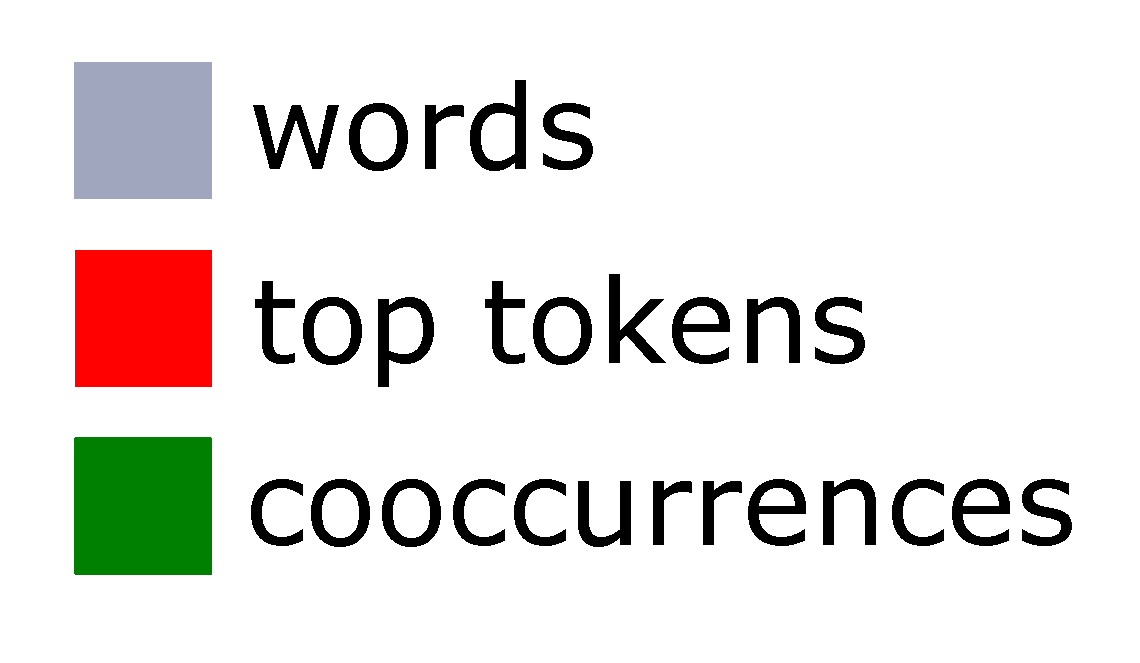
\includegraphics[width=0.25\textwidth]{legend.eps} \\
    %\end{tabular}
    \caption{Демонстрация доли текста, покрытой верхними словами, на примере одного документа. Словопозиции обозначены серо-синим цветом, словопозиции верхних слов показаны красным цветом, зелёным цветом показаны словопозиции, имеющие ненулевой вклад в расчёт когерентности (т.е. попадающие в скользящее окно вместе с другим верхним словом).}
\label{fig:ch3_doc_compound_auto}
\end{figure}

Также в этой главе предлагаются несколько мер качества, основанных на идее \textit{внутритекстовой когерентности}.
Традиционные меры когерентности сначала выделяют какое-то множество слов по их $\phi_{wt}$ и затем анализируют, каким образом эти слова встречаются в тексте (\emph{от темы к тексту}). В предлагаемом же методе сначала выделяются все соседние слова текста, распределение $\phi_{wt}$ которых затем анализируется (\emph{от текста к теме}).

Предполагается, что этот метод будет отражать коллекцию в большей степени, нежели традиционные меры когерентности. Эксперимент на полусинтетической коллекции показывает, что предлагаемый подход действительно отличается большей чувствительностью.

\underline{\textbf{В четвёртой главе}} рассматриваются способы увеличения интерпретируемости тематических моделей. Предложен метод подбора коэффициентов сглаживания, коэффициентов разреживания и весов дополнительных модальностей при помощи математического аппарата \textit{относительных коэффициентов}.

Эта техника облегчает построение тематических моделей, все темы которых различны и не <<испорчены>> большим числом неинформативных токенов (слов общей лексики). Также она позволяет перенести имеющуюсся стратегию обучения тематической модели на
другие текстовые коллекции схожей структуры.

Также в этой главе изучается псевдорегуляризатор, основанный на допущении о функциональной зависимости $\Theta = f(\Phi)$. 
Поведение предложенного алгоритма исследуется на реальных текстовых коллекциях. Результаты показывают, что этот псевдорегуляризатор повышает ряд критериев качества и успешно комбинируется с другими регуляризаторами.

\underline{\textbf{Пятая глава}} посвящена библиотеке TopicNet. TopicNet --- открытая надстройка над библиотекой BigARTM, предоставляющая более удобные
возможности для подбора гиперпараметров, для работы с пользовательскими
регуляризаторами и для визуализации тематических моделей. Описанная библиотека доступна онлайн на GitHub.

Главная мотивация TopicNet --- создать инструмент, удобный как для новичков, так и для продвинутых пользователей. Большое внимание уделяется удобству работу и наличию <<рецептов>>, показывающих хорошее качество без трудоёмкой настройки. Численный эксперимент показывает, что TopicNet с настройками <<по умолчанию>> превосходит аналогичную библиотеку GenSim с настройками <<по умолчанию>> по критериям различности, когерентности и информативности тем.

\underline{\textbf{В шестой главе}} рассматривается задача создания таксономии коллекции диалогов контактного центра без наличия разметки. Предлагается регуляризованная тематическая модель, играющая роль первого приближения к структуре коллекции.

Предлагаемая модель является двухуровневой, то есть состоит из двух <<обычных>> тематических моделей. Модель первого уровня и модель второго ориентируются на различные признаки. Это связано с тем, что первый уровень иерархии предназначен для определения предмета диалога, а цель второго уровня иерархии --- нахождение действий, которые пытается предпринять пользователь. Существительные имеют большое влияние на темы первого уровня, а для тем второго уровня более важную роль играют глаголы.

Одна и та же стратегия обучения успешно применяется к двум разным коллекциям диалогов. Первая коллекция состоит из диалогов клиентов с представителями различными государственных организаций, а вторая представляет собой логи технической поддержки провайдера. Механизм относительных коэффициентов позволил успешно перенести веса модальностей, подобранные на первой коллекции, на вторую коллекцию.


\FloatBarrier
\pdfbookmark{Заключение}{conclusion}                                  % Закладка pdf
В \underline{\textbf{заключении}} приведены основные результаты работы, которые заключаются в следующем:
%% Согласно ГОСТ Р 7.0.11-2011:
%% 5.3.3 В заключении диссертации излагают итоги выполненного исследования, рекомендации, перспективы дальнейшей разработки темы.
%% 9.2.3 В заключении автореферата диссертации излагают итоги данного исследования, рекомендации и перспективы дальнейшей разработки темы.
\begin{enumerate}[beginpenalty=10000] 
\item 
    Методология построения аддитивно регуляризованных тематических моделей, обеспечивающая формирование <<рецептов моделирования>> с автоматизированным подбором гиперпараметров по множеству критериев и отличающаяся использованием относительных коэффициентов регуляризации и кубов гиперпараметров. 
\item 
    Архитектура библиотеки TopicNet, обеспечивающая программную реализацию данной методологии и отличающаяся использованием удобного языка описания кубов гиперпараметров и возможностью создания пользовательских регуляризаторов и метрик качества на языке Python.
\item 
    Универсальный рецепт моделирования, обеспечивающий многокритериальный выбор тематических моделей для широкого класса задач, отличающийся предварительной настройкой куба гиперпараметров по набору разнородных задач тематического моделирования.    
\item 
    Программная реализация нового критерия когерентности, обеспечивающая его эффективное вычисление и отличающееся более полным использовании данных о сочетаемости слов внутри текстовых документов.
%\item 
%    Программная реализация псевдорегуляризатора в библиотеке TopicNet, обеспечивающего быстрое однопроходное вычисление тематических векторных представлений документов и улучшение качества тематической модели по множеству критериев.
\end{enumerate}


\pdfbookmark{Литература}{bibliography}                                % Закладка pdf

% При использовании пакета \verb!biblatex! список публикаций автора по теме диссертации формируется в разделе <<\publications>>\ файла \verb!common/characteristic.tex!  при помощи команды \verb!\nocite!

\ifdefmacro{\microtypesetup}{\microtypesetup{protrusion=false}}{} % не рекомендуется применять пакет микротипографики к автоматически генерируемому списку литературы
\urlstyle{rm}                               % ссылки URL обычным шрифтом
\ifnumequal{\value{bibliosel}}{0}{% Встроенная реализация с загрузкой файла через движок bibtex8
  \renewcommand{\bibname}{\large \bibtitleauthor}
  \nocite{*}
  \insertbiblioauthor           % Подключаем Bib-базы
  %\insertbiblioexternal   % !!! bibtex не умеет работать с несколькими библиографиями !!!
}{% Реализация пакетом biblatex через движок biber
  % Цитирования.
  %  * Порядок перечисления определяет порядок в библиографии (только внутри подраздела, если `\insertbiblioauthorgrouped`).
  %  * Если не соблюдать порядок "как для \printbibliography", нумерация в `\insertbiblioauthor` будет кривой.
  %  * Если цитировать каждый источник отдельной командой --- найти некоторые ошибки будет проще.
  %
  \nocite{intracoh, popov_hier, bulatov2020topicnet, thetaless}

  %% authorprogram
  \nocite{prog_cook}%
  \nocite{prog_stkc}%
  \nocite{prog_view}%
  %

  \ifnumgreater{\value{usefootcite}}{0}{
    \begin{refcontext}[labelprefix={}]
      \ifnum \value{bibgrouped}>0
        \insertbiblioauthorgrouped    % Вывод всех работ автора, сгруппированных по источникам
      \else
        \insertbiblioauthor      % Вывод всех работ автора
      \fi
    \end{refcontext}
  }{
  \ifnum \totvalue{citeexternal}>0
    \begin{refcontext}[labelprefix=A]
      \ifnum \value{bibgrouped}>0
        \insertbiblioauthorgrouped    % Вывод всех работ автора, сгруппированных по источникам
      \else
        \insertbiblioauthor      % Вывод всех работ автора
      \fi
    \end{refcontext}
  \else
    \ifnum \value{bibgrouped}>0
      \insertbiblioauthorgrouped    % Вывод всех работ автора, сгруппированных по источникам
    \else
      \insertbiblioauthor      % Вывод всех работ автора
    \fi
  \fi
  %  \insertbiblioauthorimportant  % Вывод наиболее значимых работ автора (определяется в файле characteristic во второй section)
  \begin{refcontext}[labelprefix={}]
      \insertbiblioexternal            % Вывод списка литературы, на которую ссылались в тексте автореферата
  \end{refcontext}
  
  % Невидимый библиографический список для подсчёта количества внешних публикаций
  % Используется, чтобы убрать приставку "А" у работ автора, если в автореферате нет
  % цитирований внешних источников.
  % \printbibliography[heading=nobibheading, section=1, keyword=biblioexternal]%
  }
}
\ifdefmacro{\microtypesetup}{\microtypesetup{protrusion=true}}{}
\urlstyle{tt}                               % возвращаем установки шрифта ссылок URL
